\chapter{Basic Concepts of Deep Learning}

In recent years, artificial intelligence (AI) and deep learning (DL) have transformed the way we approach some of the most complex challenges in hydrology, geoscience, and environmental science. These technologies have moved beyond simple predictions to achieve groundbreaking feats, such as NASA’s DL-based models for real-time global precipitation estimates and large-scale climate simulations that capture fine-grained details of weather extremes. Researchers have even developed AI-driven systems akin to generative pre-trained transformer (GPT), trained on decades of environmental data, to assist in forecasting water resource availability and identifying critical climate trends.

The promise of AI and DL in water sciences is immense. From reimagining flood preparedness with hyper-accurate early warning systems to unraveling the mysteries of groundwater depletion with global-scale models, the potential applications are as vast as they are impactful. At the same time, this field is highly competitive, with scientists racing to harness these tools to address urgent environmental issues, inform policy decisions, and secure a sustainable future.

This chapter introduces the foundational ideas of AI and DL, exploring how these tools have already reshaped water and climate sciences and the transformative possibilities that lie ahead.

\begin{figure}[!h]
    \centering
    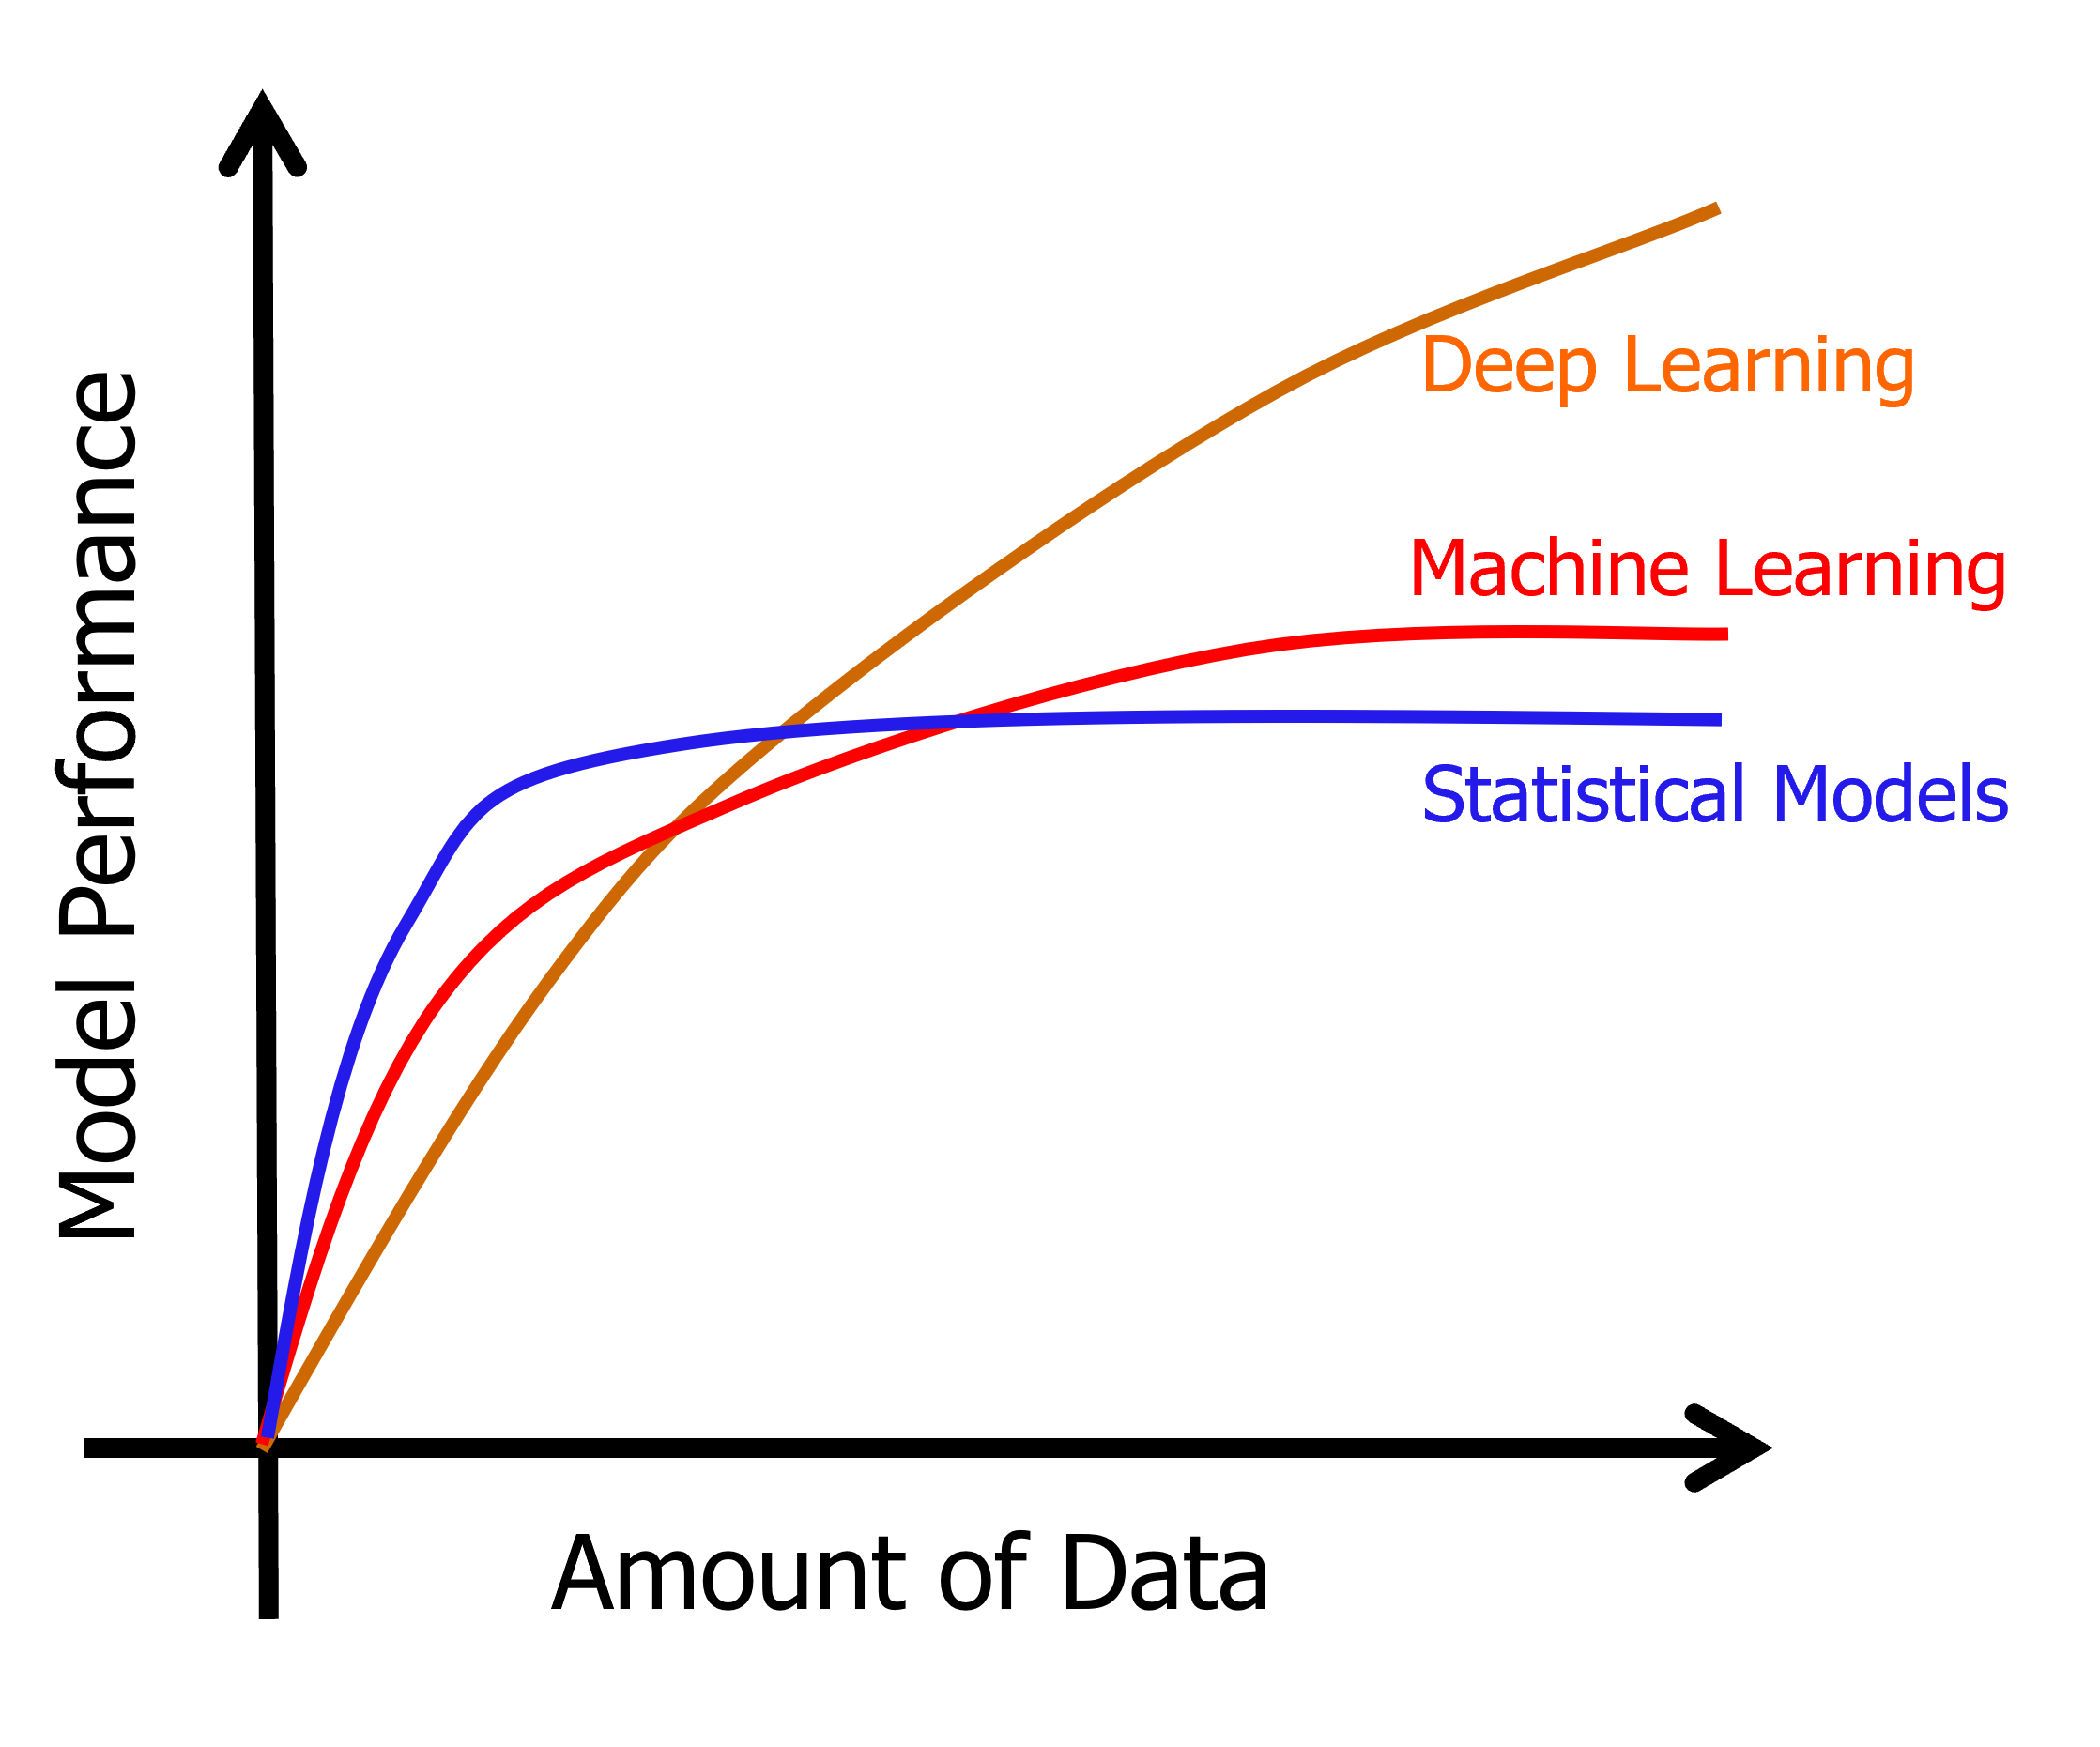
\includegraphics[width=1\linewidth]{images/What is DL.png}
    \caption{Comparison of model performance across increasing data availability for statistical models, machine learning, and deep learning}
    \label{fig:what_is_dl}
\end{figure}


\section{Understanding AI, ML, and DL: How They Relate to Each Other}
Before diving into deep learning and its applications, it’s essential to understand its roots and how it fits into the broader picture of AI and ML. Think of AI, ML, and DL as nested boxes, where each is a subset of the previous one.
\begin{figure}
    \centering
    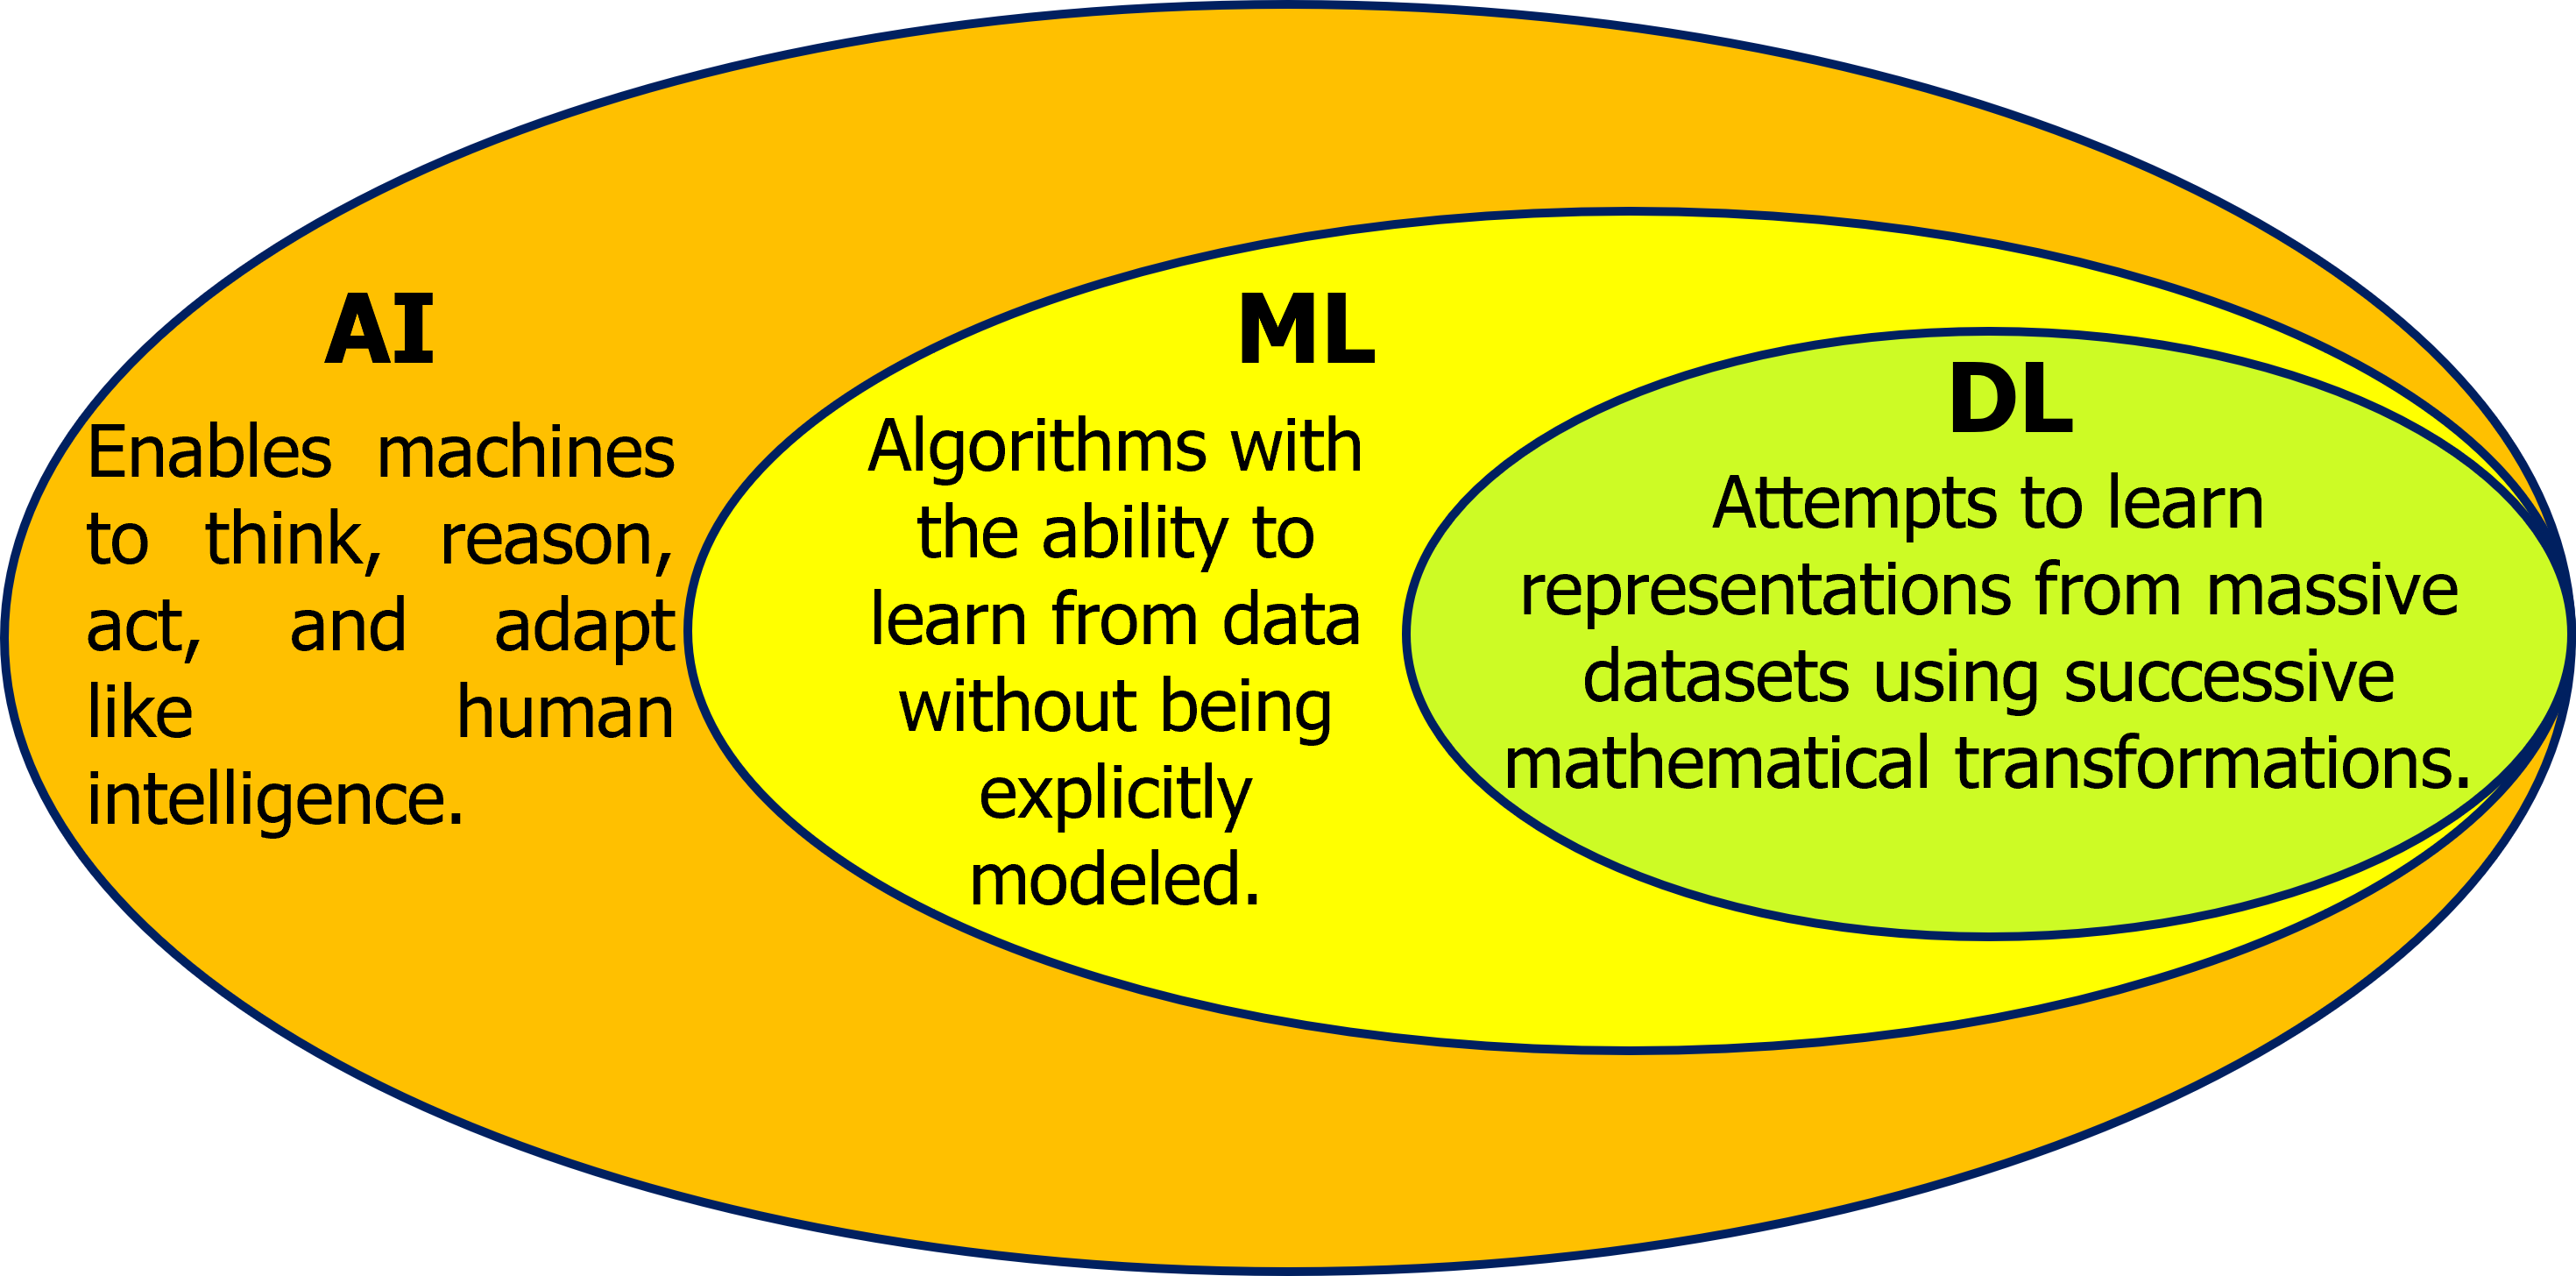
\includegraphics[width=0.99\linewidth]{images/ai-ml-dl.png}
    \caption{Illustrates the hierarchical relationship between Artificial Intelligence (AI), Machine Learning (ML), and Deep Learning (DL), with AI representing a broader field, ML as its subset, and DL as a subset of machine learning}
    \label{fig:ai-ml-dl}
\end{figure}
\subsection{Artificial Intelligence: The Big Picture}
The term Artificial Intelligence (AI) was coined in the mid-20th century, during a time when computers had only begun to show potential as tools capable of performing tasks resembling human intellect. AI broadly refers to systems designed to automate intellectual tasks typically performed by humans, such as reasoning, learning, and problem-solving.

In its earliest days, AI systems were built using hardcoded rules—a paradigm known as \textit{symbolic AI}. These systems were excellent at solving narrowly defined, logical problems, like playing chess or diagnosing straightforward faults in machinery. For example, early AI systems could be programmed to predict river discharge based on a fixed set of rules derived from historical data patterns. Another example could be simulating the operation of a water distribution network to optimize supply during drought conditions. These rule-based systems worked well for straightforward scenarios but struggled when faced with the complexity and variability of real-world problems, such as predicting extreme floods caused by unexpected climatic events.

The shortcomings of symbolic AI led to the realization that complex, fuzzy tasks—like understanding the nuances of water quality dynamics in a lake or recognizing patterns in satellite imagery of drought-stricken areas—could not be solved by explicitly defining every rule. This gave rise to new approaches like \textit{Machine Learning}, which relies on the computer learning from data rather than being explicitly programmed.

\subsection{Machine Learning(ML)}

ML emerged as a transformative step in AI's evolution. It addressed a key limitation of early AI systems, which relied on programmers explicitly defining rules for every possible situation. ML posed a new question: \textit{Could a machine learn the rules itself from data?}

This paradigm shift gave birth to a new programming approach. Instead of explicitly instructing machines, ML systems learn by example. Humans supply \textbf{input data} and the corresponding \textbf{desired outputs}, and the machine learns to infer the rules that map the inputs to the outputs. These learned rules can then be generalized to make predictions on new, unseen data. Classical programming operates as follows (see Figure \ref{fig:ml}):
\begin{enumerate}
    \item \textbf{Humans define rules} to process data.
    \item Machines apply these rules to produce outputs.
\end{enumerate}

Machine learning, on the contrary, inverts this process:
\begin{enumerate}
    \item Humans provide \textbf{ data samples and their outputs}.
    \item The machine generates the rules that connect the data to its output.
\end{enumerate}
\begin{figure}
    
    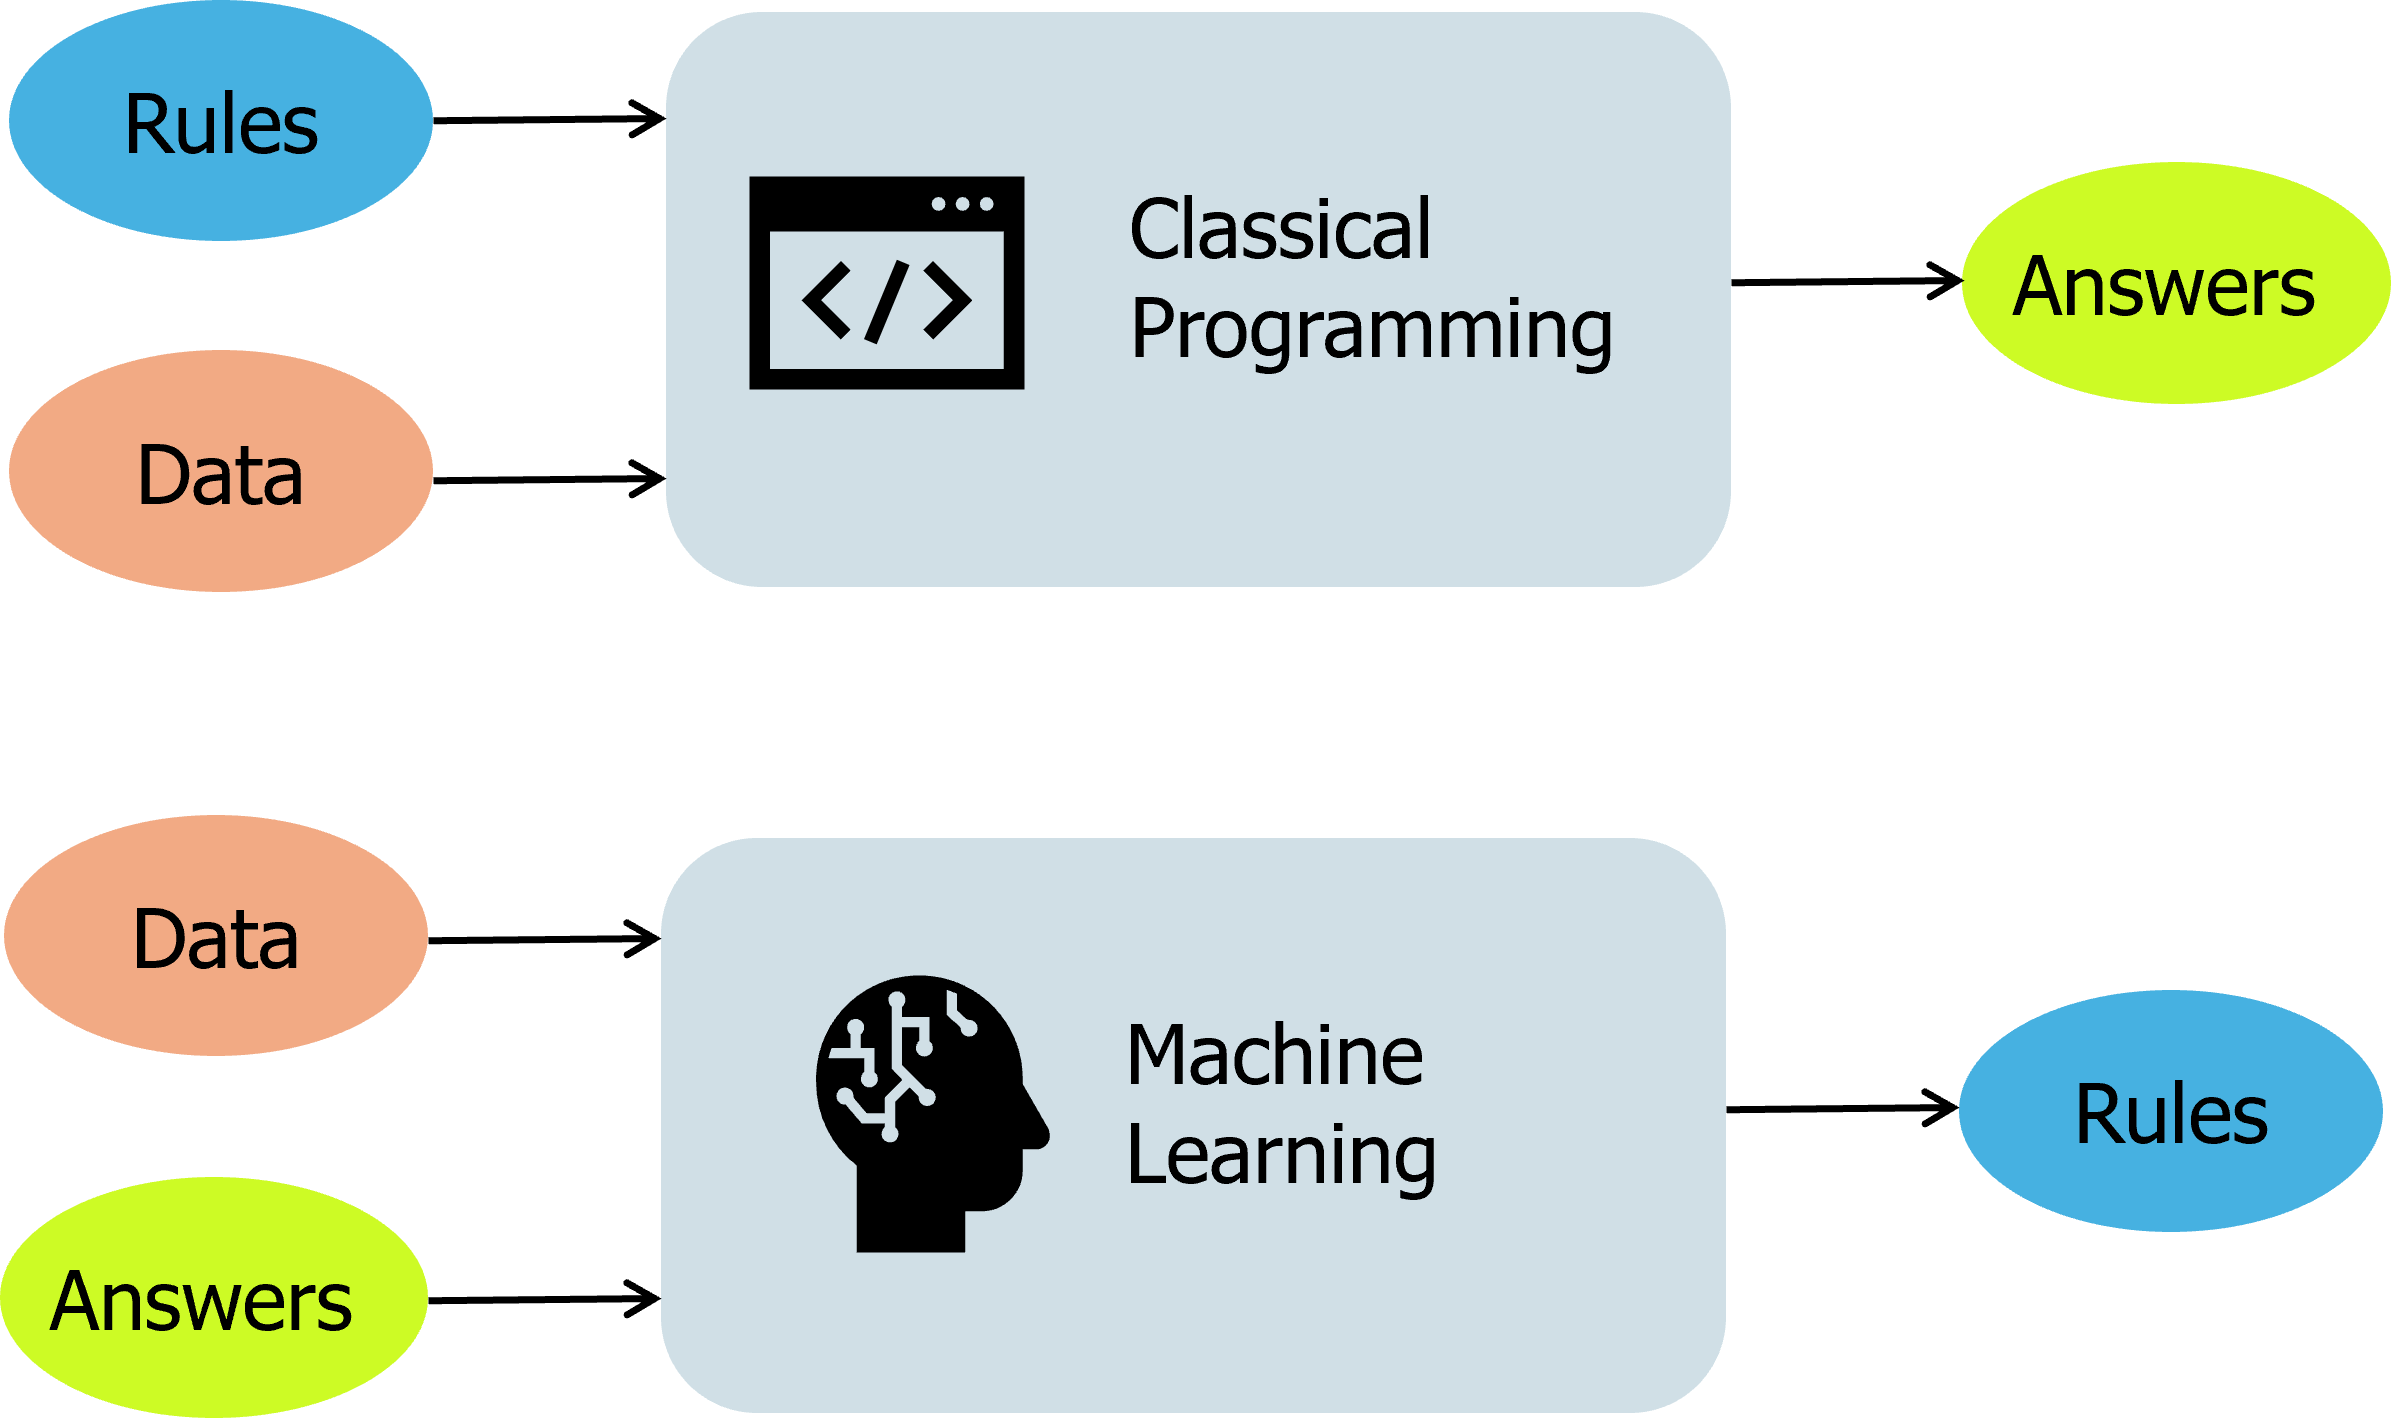
\includegraphics[width=0.75
    \linewidth]{images/ml.png}
    \caption{Classical programming vs Machine Learning (ML)}
    \label{fig:ml}
\end{figure}
This shift is similar to teaching a student by showing examples rather than lecturing about every concept. The result is a machine that can adapt and improve its performance without human intervention in the crafting of detailed instructions.

\subsubsection{Example from Hydrology}

To automate \textit{streamflow prediction}, classical programming might involve encoding complex hydrological models with explicit equations for runoff and infiltration. However, this approach struggles with unmodeled phenomena such as sudden changes in land use or climate variability.

With ML, the system is fed:
\begin{itemize}
    \item Historical data \textbf{ of rainfall and runoff} (input).
    \item Corresponding observed \textbf{streamflow values} (output).
\end{itemize}

The machine learns patterns and relationships within these data, creating a model capable of predicting stream flow under new rainfall scenarios without being explicitly programmed for every possible condition.

\subsection{Why ML Became So Popular in hydrology?}
Machine learning began to flourish in the 1990s, especially in the computer vision domain. However, its adoption in hydrology gained significant traction around 2005 and surged post-2010 due to the following factors:
\begin{itemize}
    \item \textbf{Proliferation of Diverse and Large Datasets:} Hydrology has seen an exponential increase in data availability, thanks to advancements in remote sensing technologies such as MODIS and GRACE, ground-based sensors, and climate model simulations. These multi-source, multi-scale datasets encompass high-resolution spatial and temporal data, enabling the study of nonlinear interactions across hydrological processes. ML capitalizes on such rich datasets to extract patterns and insights that traditional methods often fail to capture.
    \item \textbf{Breakthroughs in Computational Power:} The advent of high-performance computing resources, particularly GPUs (e.g., NVIDIA’s CUDA-enabled GPUs), has transformed the computational landscape. These technologies allow for efficient training of ML models on vast hydrological datasets, enabling simulations and analyses such as flood modeling, soil moisture estimation, and runoff prediction at resolutions that were once computationally prohibitive.

    \item \textbf{Capability to Handle Complexity:} Hydrological systems are inherently complex and governed by nonlinear interactions across multiple scales. Traditional statistical methods often struggle to model such complexity effectively. Machine learning, with its ability to process high-dimensional data and uncover hidden relationships, provides robust tools for prediction and inference in hydrological contexts, including flood forecasting, drought prediction, and water quality assessment.
    
    \item \textbf{Advances in Open-Source Tools and Libraries:} The widespread availability of open-source machine learning libraries like TensorFlow, PyTorch, and Scikit-learn has democratized ML adoption in hydrology. These tools make it easier for researchers to build, train, and deploy sophisticated models without requiring extensive programming expertise.

    
\end{itemize}

\section{How Machine and Deep Learning Models Learn Patterns from Data?}
To understand how ML and DL models learn, we first need to grasp the essence of learning in this context: identifying the relationship between input and output in a supervised learning pattern. At its core, learning involves finding patterns and relationships in data by optimizing representations through feedback. Let’s break this process down into key components:

\begin{itemize} \item \textit{Input Data:} The starting point of any ML task is the input data. For example, in a rainfall-runoff modeling task, the input data could include rainfall intensity, soil moisture levels, and catchment characteristics such as slope or land cover. This data serves as the foundation for predicting runoff rates.

\item \textit{Expected Output:} ML models require a target or expected output to learn effectively. For instance, the output for a rainfall prediction task might be the actual rainfall recorded, while for a flood classification task, the expected output could be labeled as “low risk” or “high risk.”

\item \textit{Feedback Mechanism:} Models need a way to measure their performance, typically through a loss function. The loss function measures the discrepancy between the model’s predictions and the actual outputs. This feedback guides the model to refine its predictions by iteratively adjusting its parameters.
\end{itemize}

\begin{tcolorbox}[enhanced,
  watermark opacity=0.3,watermark zoom=0.9,
  colback=blue!5!white, colframe=blue!70!black,
  fonttitle=\bfseries, title=Rainfall-Runoff Modeling]
  Rainfall-runoff modeling is a fundamental problem in hydrology. It involves predicting how much runoff (the water flowing over the land surface) is generated from rainfall events. This process is influenced by multiple factors such as soil moisture, land cover, topography, and precipitation intensity. By understanding these inputs and their relationship to runoff, hydrologists can better predict flood events, design infrastructure, and manage water resources.
\end{tcolorbox}







\section{The advent of Deep Learning (DL)?}
Deep learning, a specialized branch of machine learning, began gaining traction in the early 2010s as researchers sought ways to address the limitations of traditional ML models when dealing with vast and complex datasets. Unlike traditional ML, which often relies on feature engineering and shallow architectures, deep learning leverages multi-layered neural networks to automatically extract hierarchical features from data. This ability to capture complex patterns and interactions makes it uniquely suited to handle the high-dimensional and nonlinear nature of hydrological systems.

The pioneers of deep learning, such as Geoffrey Hinton, Yann LeCun, and Yoshua Bengio, introduced breakthroughs like convolutional neural networks (CNNs) and recurrent neural networks (RNNs), which transformed fields like computer vision and natural language processing. These advancements laid the groundwork for applying deep learning to hydrology, enabling innovations such as real-time flood prediction, groundwater mapping, and drought assessment.

One of the critical advantages of deep learning over traditional ML is its ability to scale with data. As datasets grew in size and complexity, shallow models struggled to generalize and required significant manual effort in feature extraction. In contrast, deep learning models excelled by learning features directly from raw data, such as satellite imagery or climate simulations. The advent of transformative architectures like transformers, which power tools like GPT, further demonstrated deep learning’s versatility and potential.

In hydrology, deep learning’s success is evidenced by applications such as predicting streamflow dynamics using long short-term memory (LSTM) networks or using CNNs for high-resolution rainfall estimation. These methods not only improve accuracy but also uncover insights into underlying hydrological processes. As computational resources and datasets continue to expand, deep learning promises to unlock new frontiers in hydrology and beyond.

\section{How Deep Learning Works: a Step-by-Step Guide}
Deep learning involves mapping inputs to outputs using a sequence of learned transformations. For example, in rainfall-runoff modeling, the input might be rainfall and soil characteristics, and the output is the amount of runoff generated. The goal of deep learning is to find a series of transformations that correctly map the input data to the output. Let’s break down how this process works in a simple and intuitive way. There are basically 3 key stages: forward pass, loss calculation, and backpropagation
\subsubsection*{\textit{Forward pass}}
Deep learning models are built using layers, and each layer transforms the input data into something slightly more meaningful (Figure \ref{fig:dl_mech1}). The specific transformation performed by a layer is determined by its weights. Weights are numbers that the model adjusts during training to improve its predictions. At the start of training, these weights are assigned random values, so the model initially produces random, nonsensical outputs.


\begin{figure}[h]
    % \centering
    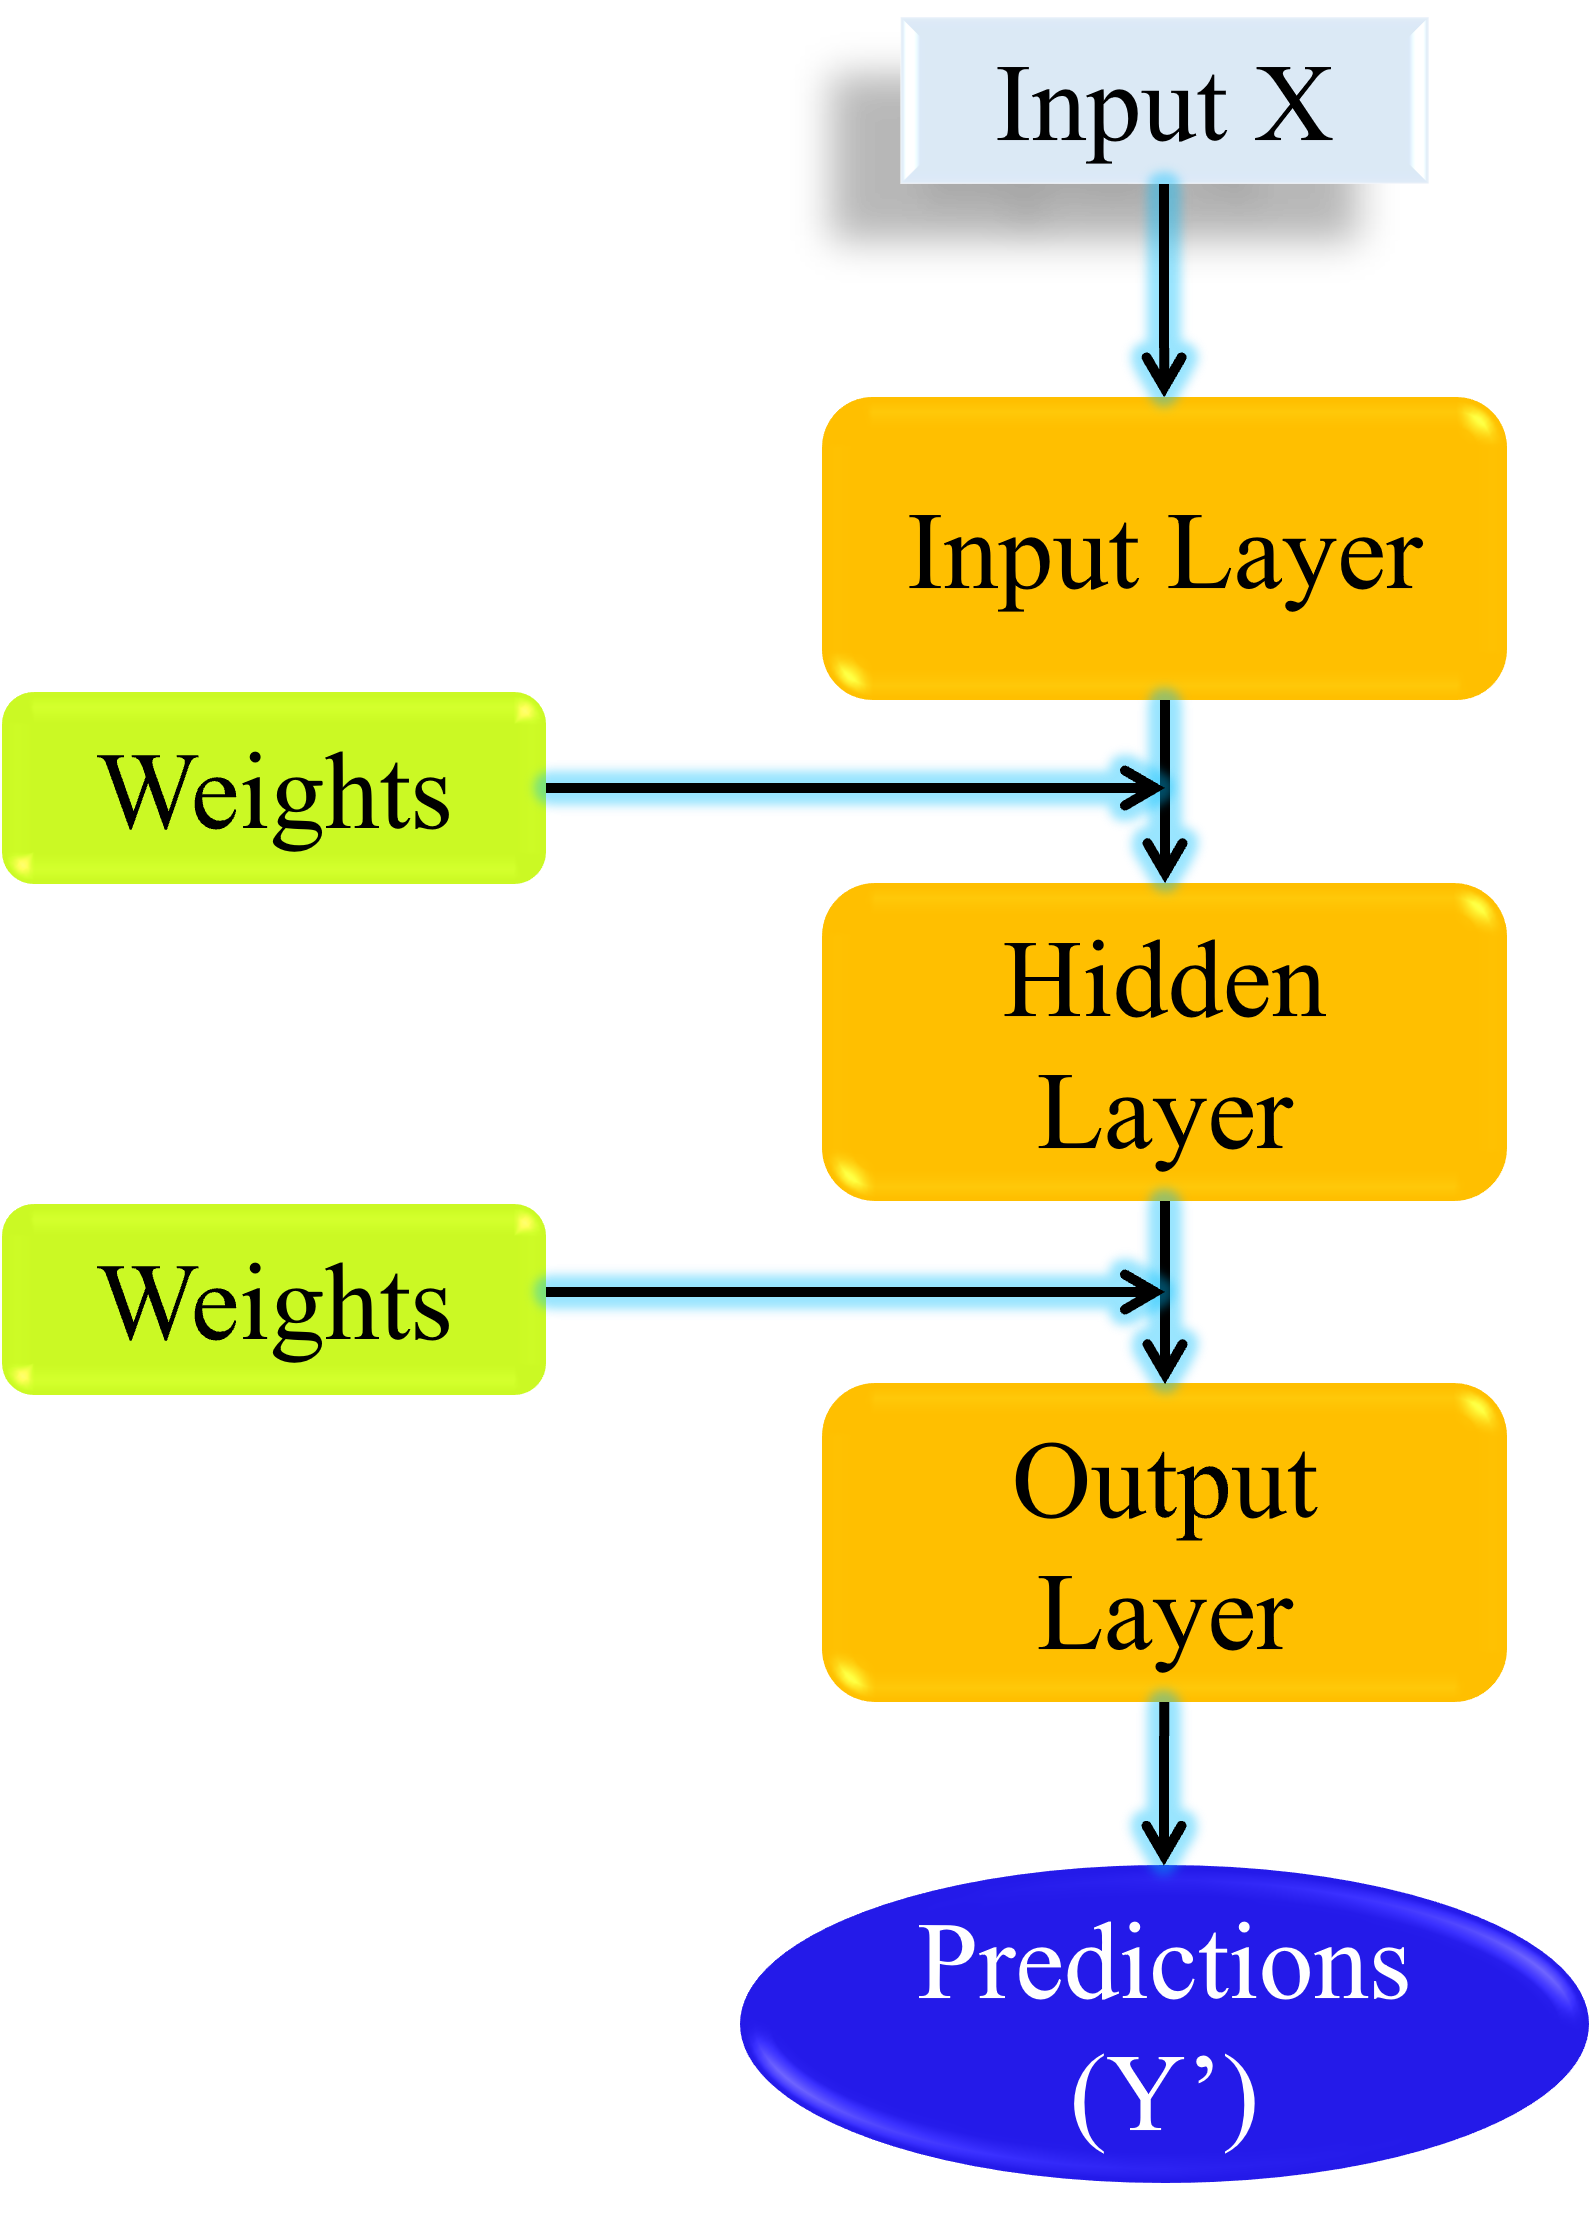
\includegraphics[width=0.4\linewidth]{images/dl_mechanism1.png}
    \caption{A deep learning model consists of a series of layers, each defined by weights that transform input data into meaningful representations.}
    \label{fig:dl_mech1}
\end{figure}
For instance, if the input to the model is rainfall intensity and the output is runoff, the first layer might perform a very basic transformation, such as amplifying the input by a random factor. Layers deeper in the model then combine these outputs into more complex patterns. The result is a series of transformations, each one building on the last, to produce the final prediction.

\subsubsection*{\textit{Loss calculation}}
To improve its predictions, the model needs a way to measure how far off its outputs are from the true values (Figure \ref{fig:dl_mech2}). This is the job of the loss function. The loss function calculates a score that represents the difference between the predicted output and the actual target. For example, if the model predicts 100 cubic meters of runoff when the actual value is 120 cubic meters, the loss function will assign a penalty to this error.
\begin{figure}[h]
    \centering
    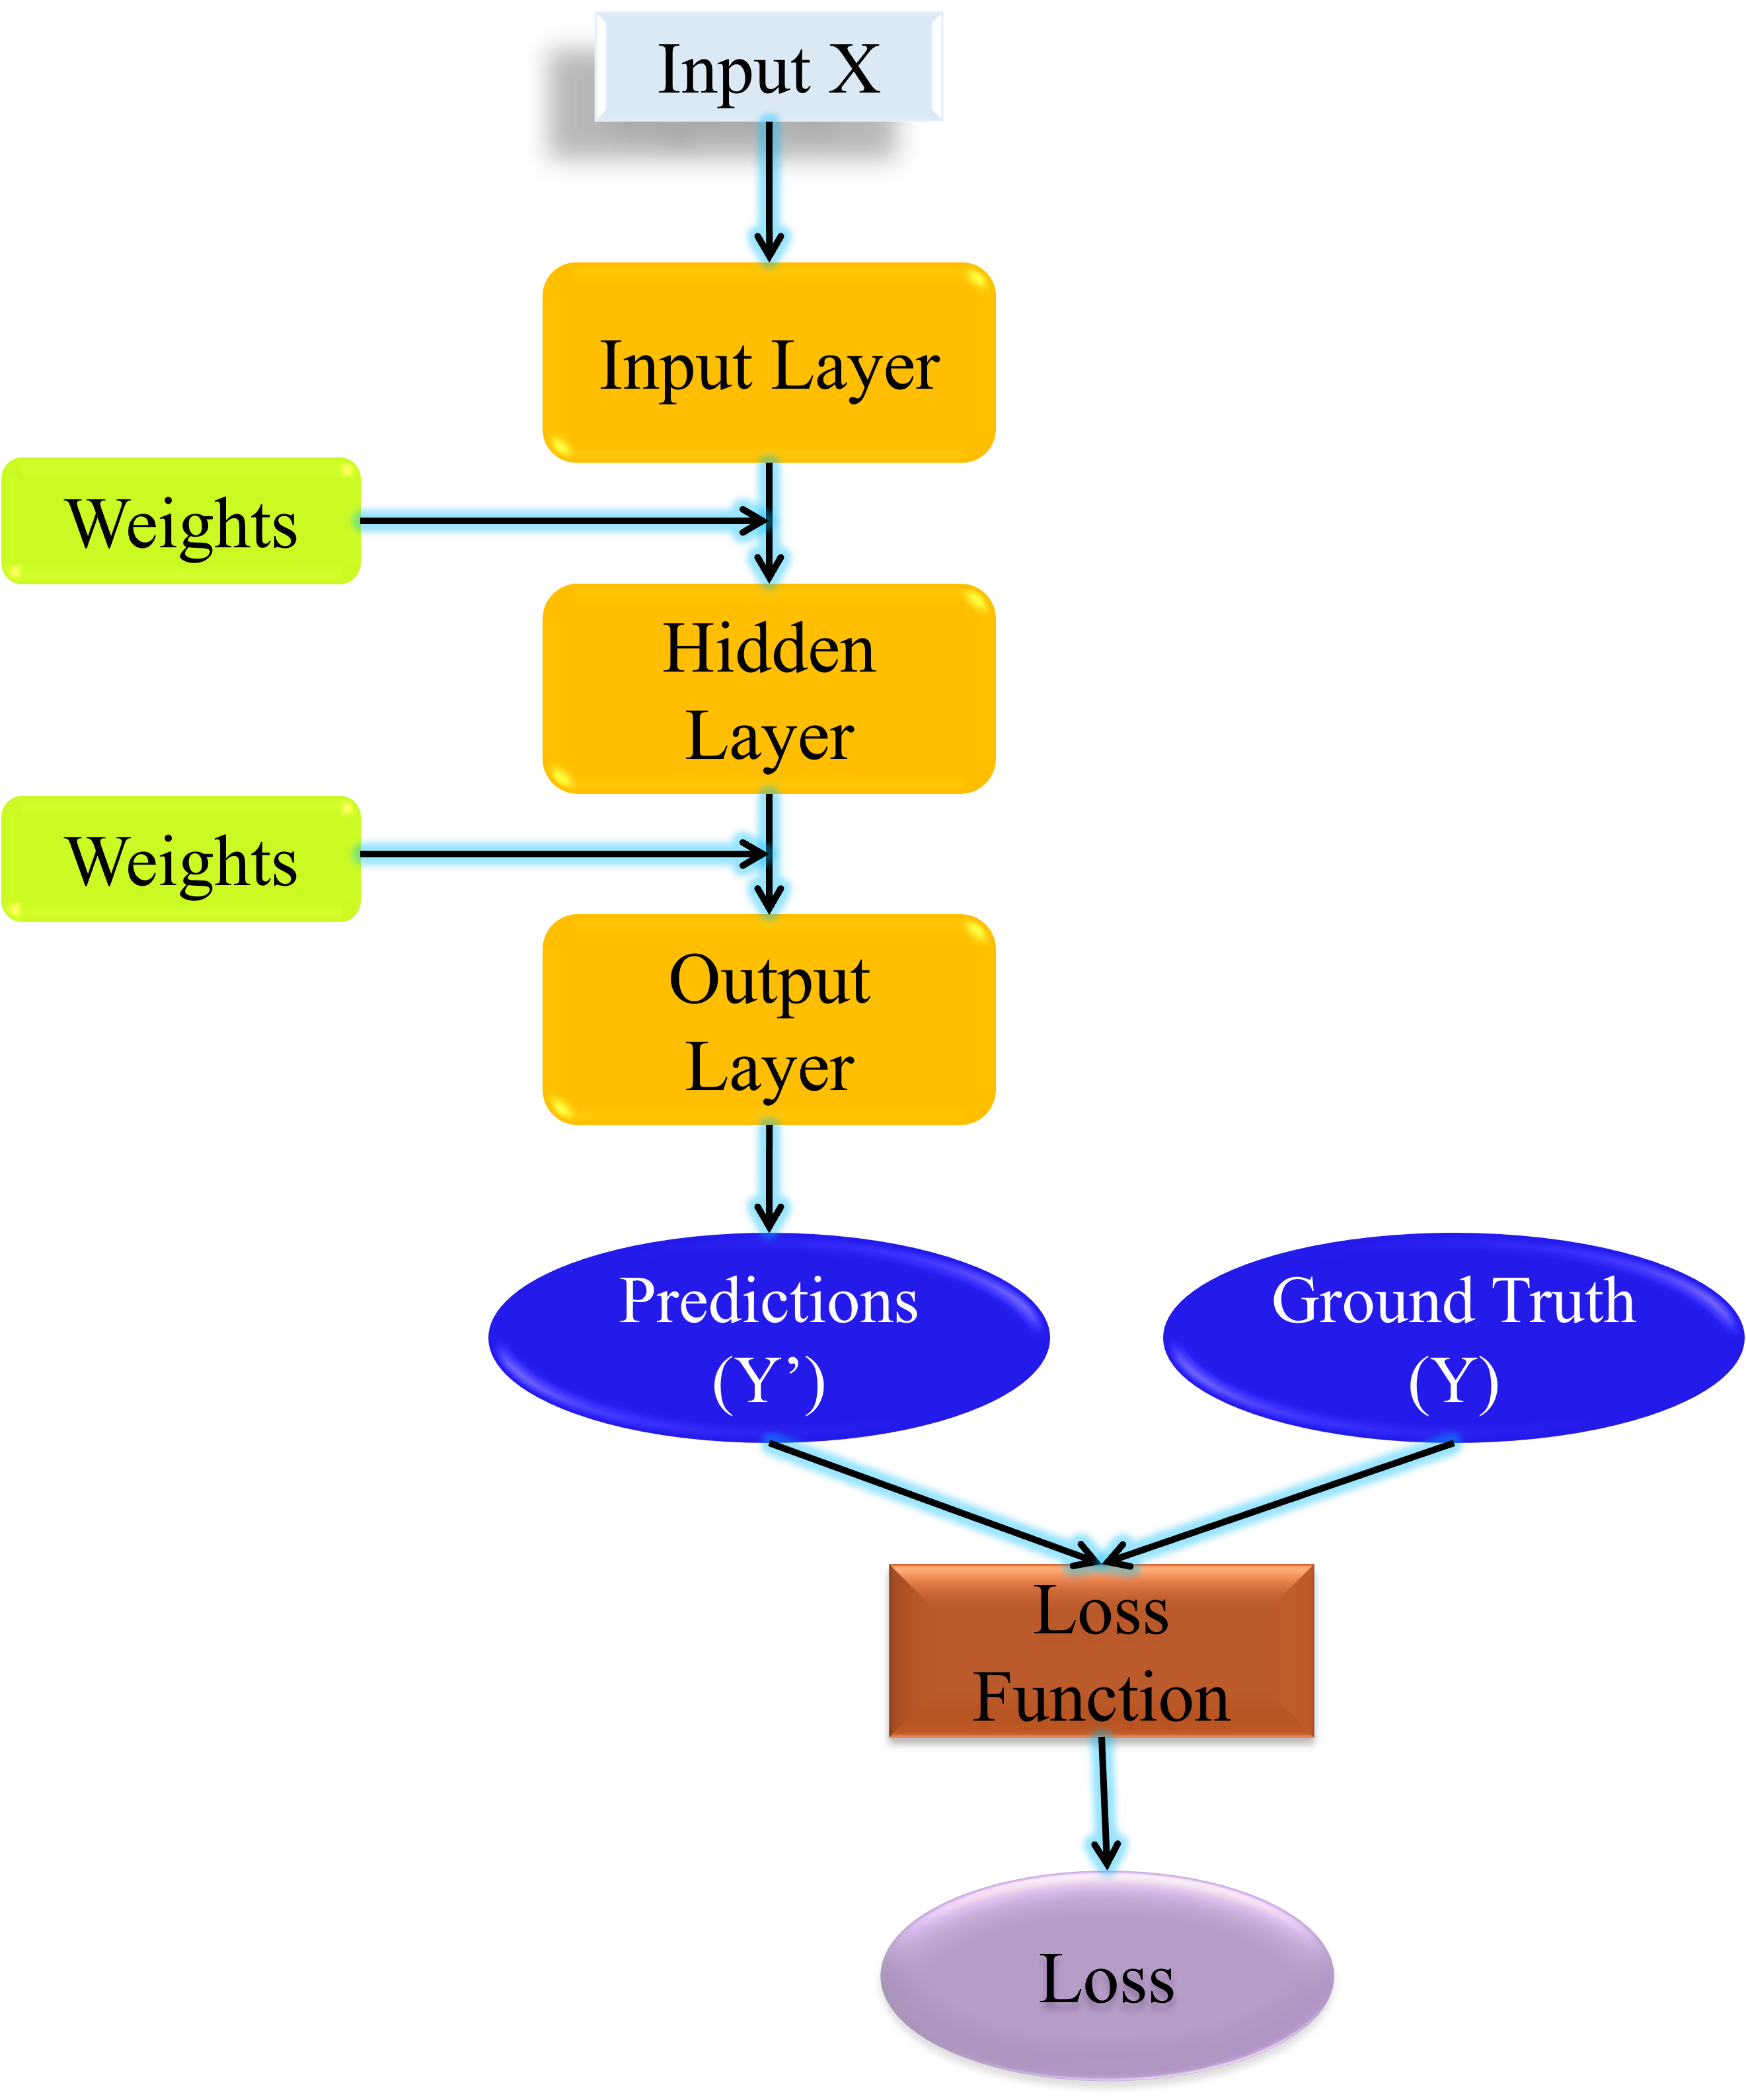
\includegraphics[width=0.4\linewidth]{images/dl_mech2.png}
    \caption{The loss function evaluates how well the model's output aligns with the target, guiding improvements through feedback.}
    \label{fig:dl_mech2}
\end{figure}
The loss function acts like a compass, pointing the model toward better predictions. The smaller the loss, the closer the model’s predictions are to the true values.
\subsubsection*{\textit{Backpropagation}} 
Once the model knows how far off it is (through the loss function), it uses this feedback to adjust its weights. This adjustment is done using an algorithm called \textit{backpropagation}, which works with an optimizer (Figure \ref{fig:dl_mech3}). The optimizer takes the loss score and calculates how each weight in the network contributed to the error. It then adjusts the weights in a way that reduces the loss.
\begin{figure}[h]
    \centering
    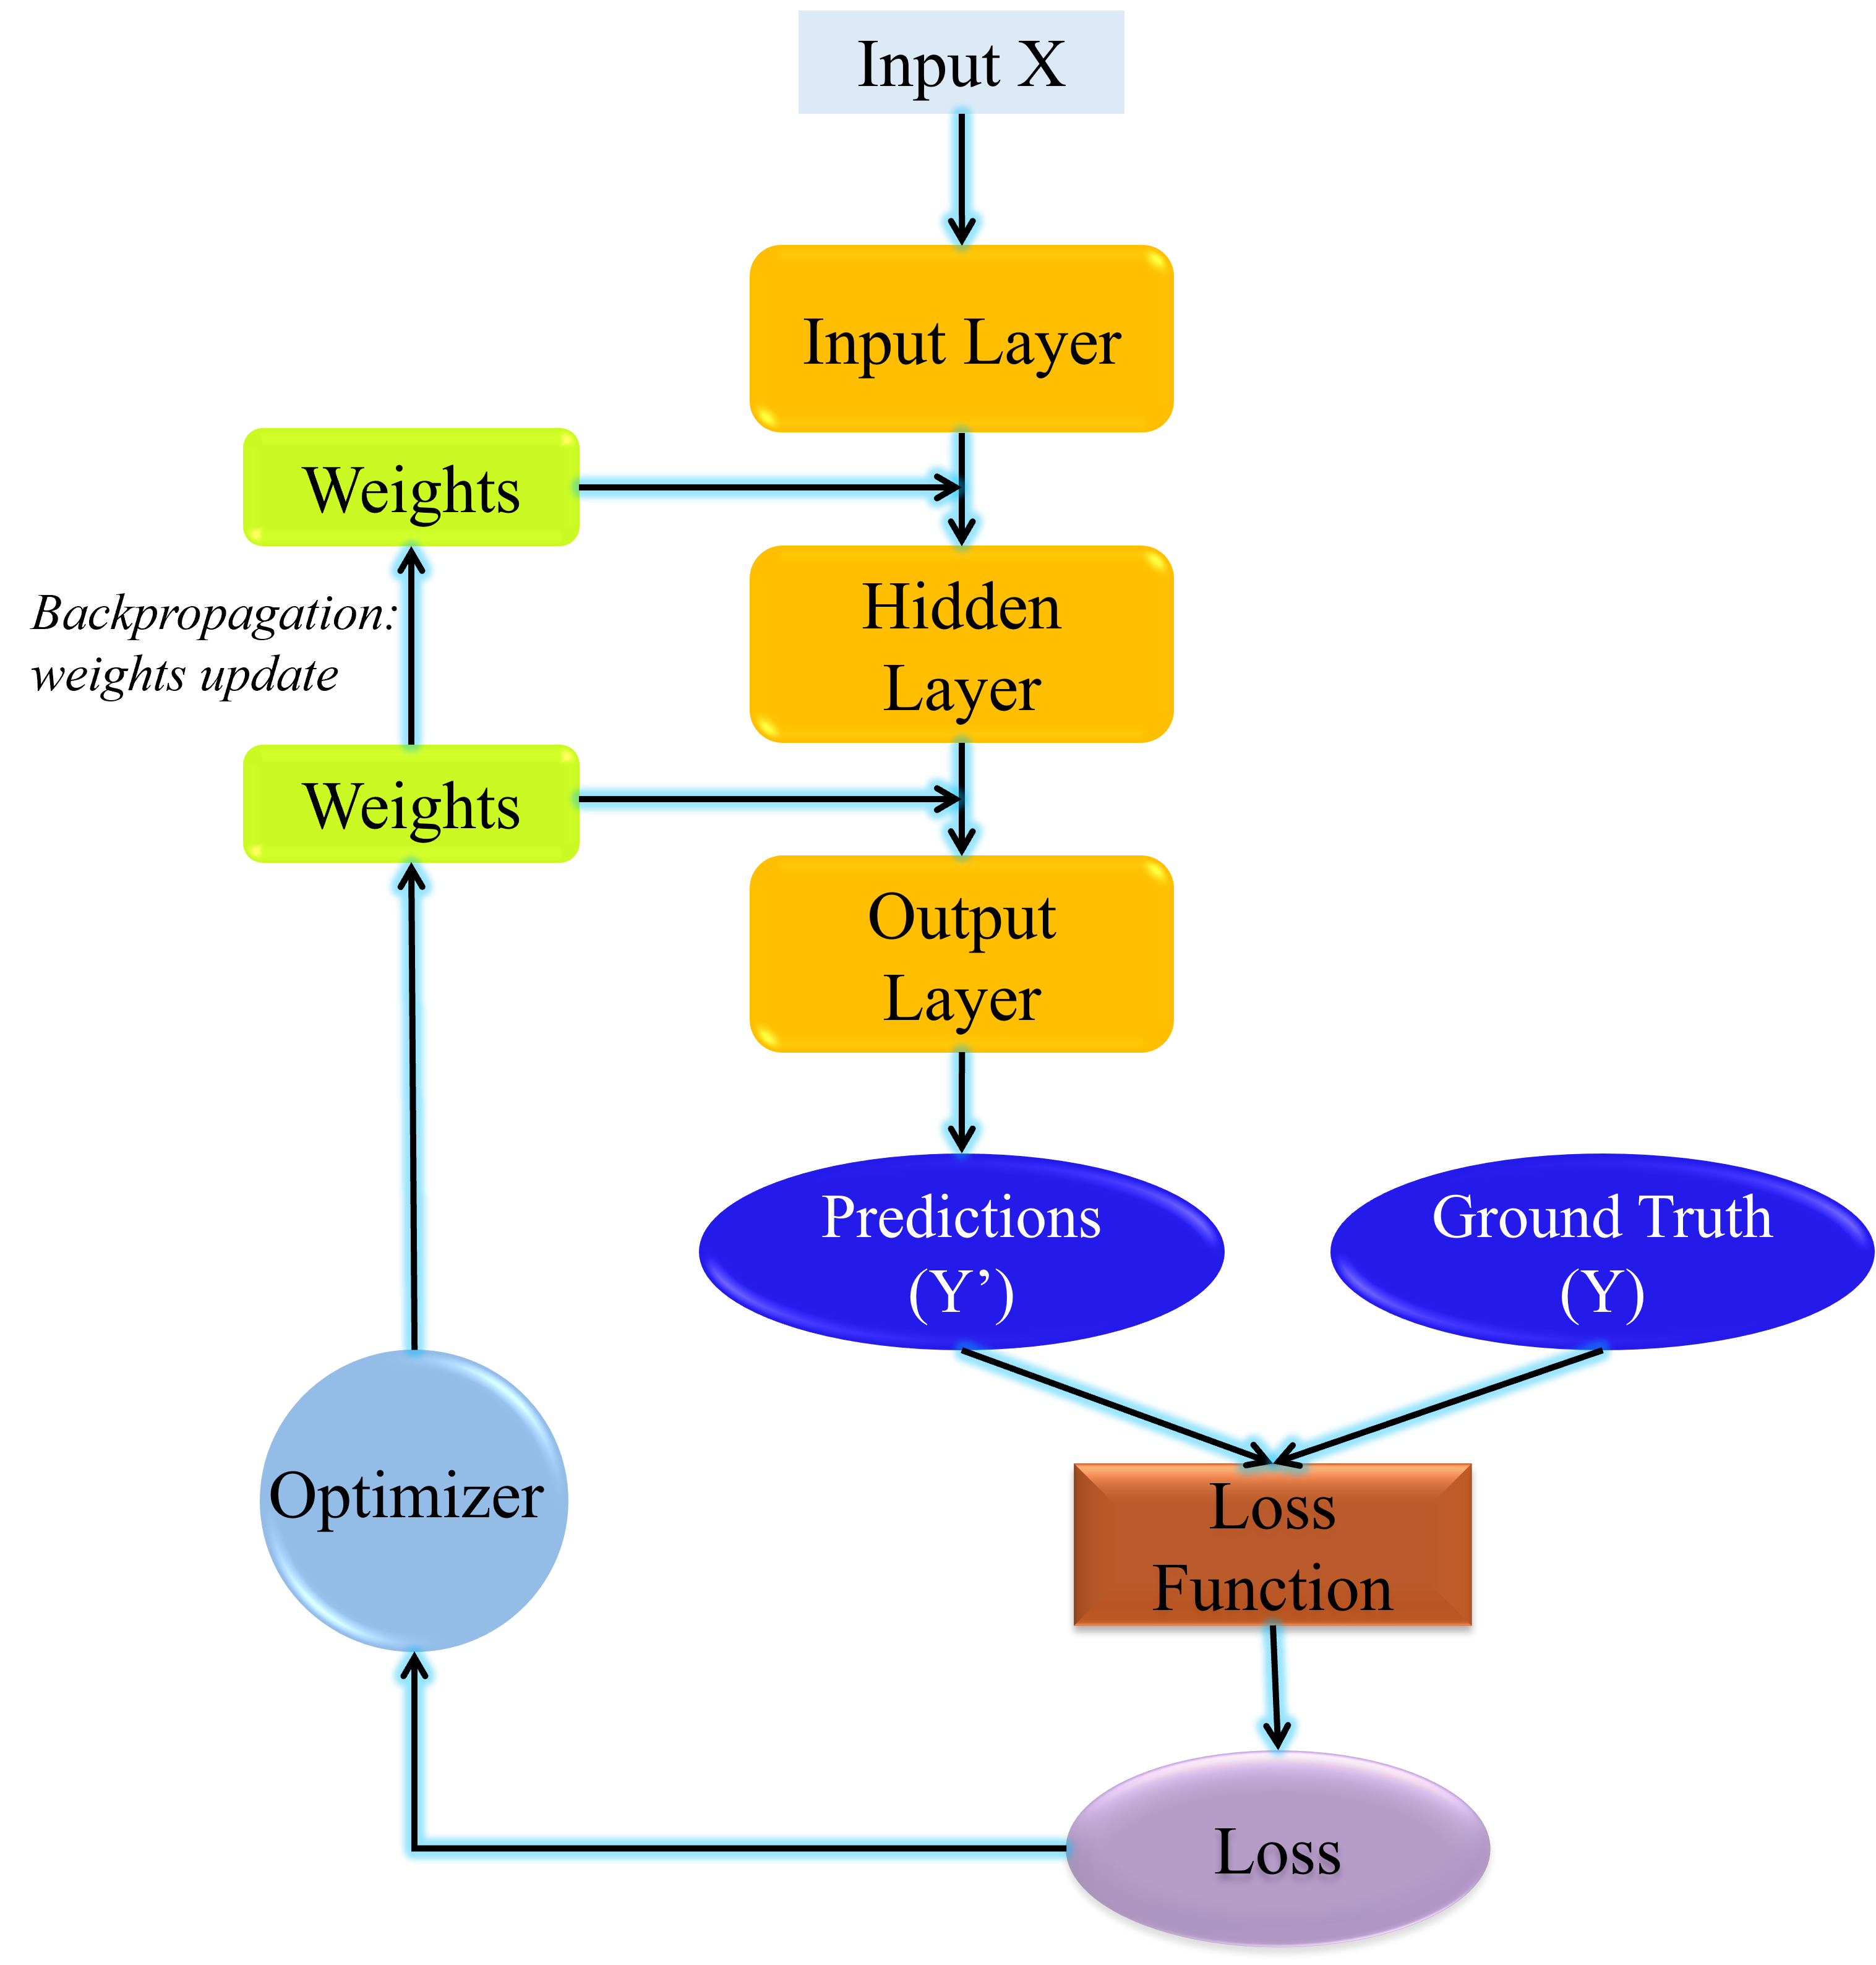
\includegraphics[width=0.7\linewidth]{images/dl_mech3.png}
    \caption{The loss score serves as feedback to adjust the model's weights through optimization and backpropagation, improving predictions with each iteration.}
    \label{fig:dl_mech3}
\end{figure}
Here’s how it works:
\begin{itemize}
    \item \textit{Prediction:} The model processes an input and produces an output using its current weights.
    \item \textit{Loss Calculation:} The loss function compares the model’s output to the true target and calculates a loss score.
    \item \textit{Backpropagation:} The optimizer calculates how to tweak each weight to reduce the loss.
    \item \textit{Parameter Update:} The weights are updated slightly in the direction that reduces the loss.
    \end{itemize}
This process is repeated for every example in the dataset, and the weights are adjusted gradually. Over time, the model’s predictions become more accurate, and the loss decreases.

\section{Regularization: Why We Need It}
As of now, you’ve learned that deep learning models can fit complex patterns in data, thanks to their multiple layers and intricate architectures. But let me ask you this: can a model be too good at fitting the data? Surprisingly, yes!

\subsubsection{\textit{The Tug-of-War Between Underfitting and Overfitting}}
instead of apples and oranges you need to explain it interms of tiug-of war also.. since we wrote that in the title.. apples and oranges are fine.. but make it better
Imagine you’re trying to teach a toddler to recognize apples and oranges. If you only tell them, “Apples are round and red,” they might struggle with oddly-shaped apples or green ones. This is underfitting—our description was too simple to capture the true variety of apples.

On the other hand, what if the toddler memorizes every single apple you showed them? They’ll recognize those apples perfectly but might fail with new ones. This is overfitting—the toddler focused too much on the examples instead of learning general rules about apples.

The same thing happens with machine learning models:

\begin{itemize}
    \item \textit{\textbf{Underfitting:}} The model is too simple to capture the patterns in the data. It performs poorly on both the training data and unseen data.
    \item \textbf{\textit{Overfitting:}} The model becomes too complex, capturing not just the patterns but also the noise in the training data. It excels on training data but fails miserably on new data.
    
\end{itemize}
So, how do we strike a balance? Enter regularization!
\subsubsection{Why Is Regularization Important?}
When training a deep learning model, we’re essentially trying to optimize its performance on unseen data. Without regularization, the model might get too attached to the training data and lose its ability to generalize. This is particularly critical in real-world scenarios, where the ultimate goal is to make accurate predictions on new, unseen data—not just the training set.

Here’s why regularization is a must:

\begin{itemize}
    \item \textbf{\textit{Generalization: }}Regularization helps ensure the model performs well on both the training data and new, unseen data.
    \item \textbf{\textit{Robustness:}} It reduces the model's sensitivity to noise in the training data, making it more stable.
    \item \textbf{\textit{Efficiency:}} A well-regularized model often requires fewer resources, as it avoids the pitfalls of complexity that don’t add value.
\end{itemize}

\subsubsection{How Does Regularization Work?}
Let’s simplify it. basically here.. we need to be consistent with the same tug-of-war example.. dont give much and different examples. stick to 1 example when explaining a concept.. dont always say imagine.. . Imagine a model as a mountain climber trying to find the lowest valley (the optimal solution). Without regularization, the climber might get stuck in every tiny dip (local patterns or noise). Regularization acts like a map, guiding the climber to avoid irrelevant dips and focus on finding the broadest, deepest valley.



As we progress through this book, you’ll come across different types of regularization techniques tailored to specific needs. 
\begin{tcolorbox}[enhanced,
  watermark opacity=0.3,watermark zoom=0.9,
  colback=blue!5!white, colframe=blue!70!white,
  fonttitle=\bfseries, title=\textit{Remember}]
  Regularization is about balance. It’s the art of making our models flexible enough to learn useful patterns but disciplined enough to avoid overfitting.
\end{tcolorbox}
\input{chapters/Part_1/DLconcepts/gradient descent}

\section{Outline:}  
Building Blocks of DL Models

Layers, weights, and activation functions.
Step-by-step walkthrough using a rainfall-runoff prediction example.
Training Deep Learning Models

Importance of loss functions and optimizers.
Concepts of overfitting and regularization techniques.
A Simple Neural Network Example

Provide a Python-based example to classify hydrological data (e.g., streamflow categories).

\section{Key Concepts in Deep Learning}
Neural Networks and Representation Learning

Introduction to tensor operations.
Role of weights and biases.
\subsection{Gradient Descent and Optimization}

Explain stochastic gradient descent.
Mention advanced optimizers (e.g., Adam, RMSProp).
Architectures in DL

Overview of CNNs, RNNs, LSTMs, and Transformers.
Application-specific suitability (e.g., CNNs for spatial data, LSTMs for time series).

